\documentclass[lnbip,sechang,a4paper]{svmultln}
%\documentclass[lnbip]{svmultln}


\usepackage{graphicx}

\usepackage{cite}
\usepackage{multicol} 
\usepackage{graphicx}

\usepackage{makeidx}  % allows for indexgeneration
\usepackage[utf8]{inputenc}

% \makeindex          % be prepared for an author index
%
\begin{document}
%
\mainmatter              % start of the contribution
%
\title{Sistema Recomendador de Turismo en Loja con  Tecnologías de Linked Data}
%
\titlerunning{Hamiltonian Mechanics}  % abbreviated title (for running head)
%                                     also used for the TOC unless
%                                     \toctitle is used
%
\author{Galo Stephano Celly Alvarado\inst{1} \and Pamela Fernanda Guamán Cañar\inst{2}}
%
   % abbreviated author list (for running head)
%
%%%% list of authors for the TOC (use if author list has to be modified)
\tocauthor{Galo Celly, Pamela Guamán}
%
\institute{Universidad Técnica Particular de Loja
\email{gscelly@utpl.edu.ec, pfguaman@utpl.edu.ec}
%\texttt{http://users/\homedir iekeland/web/welcome.html}
%\and
%Universit\'{e} de Paris-Sud,
%Laboratoire d'Analyse Num\'{e}rique, B\^{a}timent 425,\\
%F-91405 Orsay Cedex, France
}

\maketitle     % typeset the title of the contribution
% \index{Ekeland, Ivar} % entries for the author index
% \index{Temam, Roger}  % of the whole volume
% \index{Dean, Jeffrey}

\begin{abstract}        % give a summary of your paper
La web semántica, una web más avanzada, posee la visión de generar conocimiento a fondo ya que se comportaría como una máquina procesable e interpretable a causa de tener la capacidad de dar significado a los recursos web.  Actualmente en el Ecuador el turismo es un sector activo, que cuenta con varias fuentes de información de internet, pero lastimosamente para el turista esta información no es accesible en su totalidad debido a que estas fuentes se encuentran dispersas y no se encuentran estructuradas para ser vinculadas unas con otras, dejando al humano una gran carga para la búsqueda de información. 
En esta propuesta se pretende construir un sistema recomendador de turismo usando tecnologías de web semántica, para que la información turística pueda ser aprovechada y brindar al usuario una búsqueda mejorada.
%                         please supply keywords within your abstract
\keywords {linked data, turismo, Ecuador, Loja, twitter, sistema recomendador.}
\end{abstract}
%
\section{Introducción}

Actualmente en el Ecuador el turismo es una de las actividades económicas que aportan positivamente al país, sin embargo no es el principal sector económico ya que el petróleo tiene el primer lugar como generador de ingresos en el país.

Considerando que, en cuanto al área del turismo en el país falta mucho por explotar, en el año 2015 de acuerdo al Ministerio de Turismo de Ecuador se ha obtenido ingresos de un estimado de 1.691,2 millones de dólares  obteniendo un crecimiento promedio anual del 13 \% ~\cite{puno}, una cantidad alentadora para este sector que con  priorización de productos, de destinos y de mercados estos números podría aumentar.

El internet es la principal herramienta para las búsquedas sobre planeación de viajes de ocio o negocio con un 76\% frente a otro tipo de fuentes de información (libros, TV, revistas, agencias, radio, otros) ~\cite{pdos}. Dentro de internet, como fuentes de inspiración para viajes lideran las redes sociales, sitios de fotos o vídeos con un 83\%, por otro lado los motores de búsqueda son los siguientes de la lista con un 61\% y con porcentajes menores se encuentran las aplicaciones propias de reseñas o de viajes.

Uno de los principales inconvenientes que existe en la web actual es que la información encontrada con respecto a temas turísticos de un lugar se encuentra dividida en dos~\cite{seis}. Una parte de estos repositorios de información están en documentos de municipios o ministerios de turismo, también  se encuentra en sitios web bien estructurados propios a un individuo u organización (proveedores de viajes, agencias, etc.), y otra parte de esta información se encuentra en la misma “World Wide Web” repartida en pequeñas partes con información más detallada de las actividades o  eventos que se realizan en distintos lugares.

Para hacer frente a este problema, en este trabajo se propone diseñar un sistema recomendador inteligente con uso de  tecnologías de web semántica, que permita conectar semánticamente (integrar y enlazar datos) la información turística del Ecuador existente en la web, considerando como fuente principalmente twitter, para generar un sistema recomendador orientado al turismo.  

Esto permitirá a un usuario interesado reducir la carga de búsqueda de información turística en distintas fuentes, proporcionando facilidad y eficiencia al realizar sus consultas, además de contar información completa y relacionada (sobre hoteles, comida, eventos,etc.) que permitirá al usuario identificar su mejor destino turístico.

Por otro lado, todo tipo de empresas, comercios, en general la economía del país se beneficiarán de este proyecto, debido a que la información correspondiente a su empresa, formará parte de los datos enlazados de la web semántica y estarán disponibles para todos cibernautas que se encuentren interesados en visitar algún sitio turístico de la provincia de Loja. 

\section{Fundamentos Teóricos}

La web semántica es una extensión de la web actual, que por su información bien definida da un mayor significado a los recursos de la web brindando una búsqueda más exacta y avanzada ~\cite{siete} .

Linked data o 'datos enlazados', se refiere a conectar datos relacionados que no estén vinculados, con el fin de disminuir las barreras que hay, para enlazar los datos utilizando otros métodos ~\cite{tres}. En otras palabras se usa este término para referenciar, compartir y conectar datos, información, generando conocimiento en la web semántica usando URIs (Identificador de recursos uniformes) y RDF (Resource Description Framework).

Social networks, las redes sociales son como una comunidad virtual  que reúne a las personas para hablar, compartir ideas e intereses, o hacer nuevos amigos. Este tipo de colaboración y distribución se conoce como medios de comunicación social. A diferencia de los medios tradicionales que normalmente se crean por no más de diez personas, los sitios de redes sociales contienen contenido creado por cientos o incluso millones de personas diferentes ~\cite{pcuatro}.


\section{Objetivos}

En el presente trabajo se pretende cumplir con los siguientes objetivos:

\begin{itemize}
    \item Diseño de un modelo que permita la construcción de un sistema recomendador de turismo  basado en linked data.
    \item Integración y vinculación de datos del sector turístico de municipalidades o ministerios de turismo y twitter, para realizar búsquedas avanzadas que generen conocimiento.
    \item Construcción del sistema recomendador.
\end{itemize}

Entre los beneficiarios con la implementación de este sistema recomendador se encuentran:

\begin{itemize}
    \item El turista, que encontrará información completa y oportuna sobre información turística de interés.
    \item Las instituciones turísticas o negocios, ya que tendrán una ventaja competitiva.
    \item El país, la ciudad de Loja, visto que mejorará el índice de turismo y podrá generar mayores ingresos, y un ejemplo de modelo de datos enlazados para un sistema recomendador de turismo, que puede ser aplicado a más ciudades, además de poder enlazar más fuentes de información.

\end{itemize}

\subsection{Trabajos relacionados}

Caso de uso de Open Data y Linked Data en Turismo ~\cite{uno}, los autores analizan la ventaja competitiva que obtendrían  los sectores industriales y turísticos con un uso de tecnologías de Linked Data y Linked Open Data. La información es tomada de opiniones que los turistas han hecho en las redes sociales, lo que genera valiosa información para conocer las tendencias que los turistas tienen al visitar un lugar.

Open linked data y dispositivos móviles como una herramienta de e-turismo. Aproximación práctica para un e-learning colaborativo ~\cite{dos}, se presenta una aplicación móvil usada como una guía turística para los usuarios, la misma que permite la colaboración entre instituciones públicas y sus datos abiertos, al ser móvil siempre está disponible para añadir nuevos conocimientos sobre los distintos temas turísticos de un lugar.


LinkedQR: mejora de la experiencia turística a través de datos vinculados y códigos QR~\cite{cinco}, los autores diseñan y presenta una herramienta que permite la colaboración de los códigos QR y datos enlazados usando tecnologías móviles. La aplicación proporciona a los turistas recuperar conocimiento adicional a partir de los códigos QR  de galerías de arte o de alguna instalación turística.

Aplicación de tecnologías web semántica para los sistemas de información turística ~\cite{seis}, se menciona la importancia que tiene una búsqueda basada en web semántica, especialmente en el turismo. Un sistema de este tipo  brindaría óptimos resultados al momento de asistir un evento ya que se puede ofrecer información adicional como: ubicación, reseñas, etc. 

Un sistema recomendador móvil  para la información de los datos de la web ~\cite{diez}, se diseña SMART-MUSEUM, un sistema móvil recomendador para la web de datos y su aplicación a las necesidades de información de los turistas en contexto de acceso al patrimonio cultural. Este sistema usa lenguajes de la web semántica para representar los datos, y el uso de ontologías como puente semántico entre las descripciones de contenido heterogéneo, las entradas de sensores y los perfiles de usuario. El resultado de este proyecto demuestra que el razonamiento basado en ontologías, la expansión de consultas, el agrupamiento de resultados de búsqueda y el conocimiento del contexto brinda una mejora significativa al momento de realizar una recomendación, cumpliendo las expectativas de los usuarios. El uso de sistemas de este tipo indica que la representación y recuperación de contenido semántico mejora en gran manera el rendimiento de los sistemas de recomendación móvil.

Sistema inteligente de recomendación turística ~\cite{once}, donde presenta una encuesta detallada y actualizada sobre este campo, considerando los diferentes tipos de interfaces, la diversidad de algoritmos de recomendación existentes, las funcionalidades que brindan y el uso de técnicas de inteligencia artificial, además de proveer pautas para la construcción de recomendadores turísticos. Explotando el poder de aplicaciones de la web, tales como son las redes  sociales. Estas herramientas ayudan el uso de técnicas de filtrado colaborativo, puesto que permiten nuevas formas de calificación o recolección de información de usuarios a nivel individual o social. En el caso del turismo los usuarios tienen una nube de etiquetas asociada con términos relevantes a su perfil, esta información es usada para comparar las nubes de etiquetas de usuarios, elementos y encontrar coincidencias

Diversificación semántica de las recomendaciones turísticas ~\cite{docea}, describe varios métodos de diversificación, variaciones de métodos y un nuevo algoritmo de selección basado en la agrupación semántica, todos estos métodos probados en un recomendador de actividades turísticas. Su resultado muestra que el método cuadrático es la mejor combinación de diversidad y precisión, puesto que los bucles para todos los elementos de la lista para encontrar el elemento que combina mejor la diversidad y la exactitud, aunque no es el adecuado para ser ejecutado en tiempo real ya que sus costos de computación son muy elevados.

La siguiente actividad, conectar las visitas del museo ~\cite{doceb}, introduce una metodología para ofrecer a los visitantes otros atractivos culturales basados en sus anteriores visitas a los museos. Las preferencias de los usuarios que visiten los museos y su comportamiento es rastreado mediante una guía móvil del museo y usado para crear un modelo del visitante. Utilizando modelos semánticos y datos enlazados abiertos ayudan a la representación de activos regionales como objetos culturales tal es el caso de museos. Los modelos de los visitantes se explotan con un enfoque de similitud gráfica para identificar oportunidades personalizadas para todos los usuarios por medio del filtrado de objetos culturales que considere relevantes.

Diseño y desarrollo de RecSys en tiempo real basado en actividades de localización, dispositivos móviles y turismos ~\cite{docec}, expone un modelo novedoso para sistemas de recomendación en tiempo real para las atracciones turísticas del Reino Unido. Desarrollando una aplicación móvil para los turistas que respalde el acceso a la información filtrada de lugares que estén dentro de las atracciones turísticas como artefactos, guías, mapas, información de comercios y proveer la facilidad de compartir sus experiencias. Igualmente crearon un sistema de recomendación en tiempo real basado, basado en el seguimiento y las actividades que realizan las personas, donde se les da información de contenidos relevantes según su ubicación física. 

El presente proyecto pretende impulsar el sector turístico de la ciudad de Loja con la implementación de linked data sobre datos de instituciones turísticas y twitter. El presente sistema recomendador permitirá recolectar la información relacionada al turismo de la ciudad de Loja, principalmente de lugares turísticos, hospedaje, restuarantes,  eventos. La información de twitter será recolectada a partir de publicaciones con hashtags referentes al turismo.  La aplicación final recomendará en base al mayor número de menciones que ha tenido el recurso turístico, que una vez enlazado podrá sugerir al usuario lugares, eventos, restaurantes, entre otras alternativas que pueden ser de su agrado.

Con un sistema recomendador de turismo, no sólo se prevé una mejor experiencia en su viaje al turista, sino también a agencias turísticas o negocios que con la información enlazada en este sistema tendrán una ventaja competitiva en el mercado y así generar mayores ingresos económicos en el sector turístico.


\section{Metodología}

La metodología con la que se desarrollará el proyecto, como se muestra en la Figura \ref{fig:uno}, se la describe en las siguientes fases:

\subsection{Primera Fase: Fuentes de Datos}
Esta es la primera fase donde se buscan y analizan las posibles fuentes de información que nos proporcionan datos de los cuales podemos generar nuevos conocimientos. 

Con respecto al turismo a nivel de la provincia de Loja, se considerará como fuentes principales los datos recolectados del Ministerio de Turismo del Ecuador - Zona 7 y la red social de Twitter.

\subsection{Segunda Fase: Extracción y Limpieza}
En la segunda fase se extrae la información de las fuentes previamente seleccionadas.

Las herramientas para extraer la información será mediante el uso de el API de twitter y la librería Tweepy. Para la información turística de la provincia de Loja, se utlizará el catastro turístico del Ministerio de Turismo de Ecuador Zona 7, se extraerá información turística relevante de la provincia.


\subsection{Tercera Fase}
En esta tercera fase se modela el dominio e identifica los conceptos, clases, relaciones y propiedades necesarias.


Para modelar una ontología que modele el turismo en la provincia de Loja, se utilizará en lo posible  vocabularios referentes a este tipo de temas, como:  Cruzar y Km4city (vocabularios con dominio turístico), Schema, RDFs, entre otros.

Sin embargo se definirá un vocabulario propio que ayudará a la creación de clases y relaciones que definan de mejor la ontología. 

Los vocabularios que se utilizarán para la ontología son:
\begin{table}[htbp]
\begin{center}
\begin{tabular}{|l|l|}
\hline
Vocabulario &  URI\\
\hline \hline
Propio & http://www.semanticweb.org/sbc/turismo  \\ \hline
Km4city & http://www.disit.org/km4city/schema   \\ \hline
Cruzar & http://idi.fundacionctic.org/cruzar/turismo \\ \hline
Schema & http://schema.org \\ \hline
FOAF & http://xmlns.com/foaf/0.1/ \\ \hline
\end{tabular}
\caption{Vocabulario a utilizar}
\label{tabla:sencilla}
\end{center}
\end{table}

\subsection{Cuarta Fase: Carga y Enriquecimiento de datos}
En esta fase se realizará la transformación de los datos que se extrajo previamente en la primera fase mediante y  el modelado de la ontología de la tercera fase. 

Todos los datos obtenidos pasan a la etapa de transformación a un formato RDF, lo cual permite enriquecer aún más los datos, mediante una herramienta de creación y modelado de ontologías como Protégé.

Toda la información que ha sido transformada a este nuevo formato será guardada en un base de datos NoSql (Mongo DB), donde los datos estarán en un formato de tripletas con una URI. Esto permitirá enlazar dtaos y tener información  que sea capaz de responder preguntas que un turista normalmente tiene. 

\subsection{Quinta Fase: Explotación de Datos}
En esta fase se desarrollará una interfaz gráfica amigable al usuario o turista que le permita realizar consultas de tipo turístico. El recomendador responderá en base a la información base del catastro turístico de la provincia de Loja y los tweets recuperados.
 
\hfill \break

\begin{figure}
\centering
\includegraphics[height=14cm]{arquitectura}
\caption{Metodología}
\label{fig:uno}
\end{figure}


\section{Desarrollo}
En base a la metodología propuesta en el apartado anterior, para el desarrollo
del proyecto se especifican las actividades detalladamente en por cada fase:
\subsection{Primera Fase}

Se ha considerado tomar las siguientes fuentes de información:
\begin{itemize}
    \item Ministerio de Turismo: Catastro turístico de la Zona 7, específicamente la provincia de Loja, en el cual se encuentra información turística como: restaurantes, bares, cafeterías, discotecas, lugares que prestan servicio de alojamiento y lugares turísticos de la provincia, cada uno de estos recursos con su respectivos datos como: nombre, teléfono, dirección y coordenadas.
    \item Twitter: Es una red social donde las personas comparten ideas, reseñas, etc., en base a los tweets que las personas o turistas realizan respecto a Loja, algún evento, sitio turístico, alojamiento o comercial.
    
\end{itemize}

\subsection{Segunda Fase}
\begin{figure}
\centering
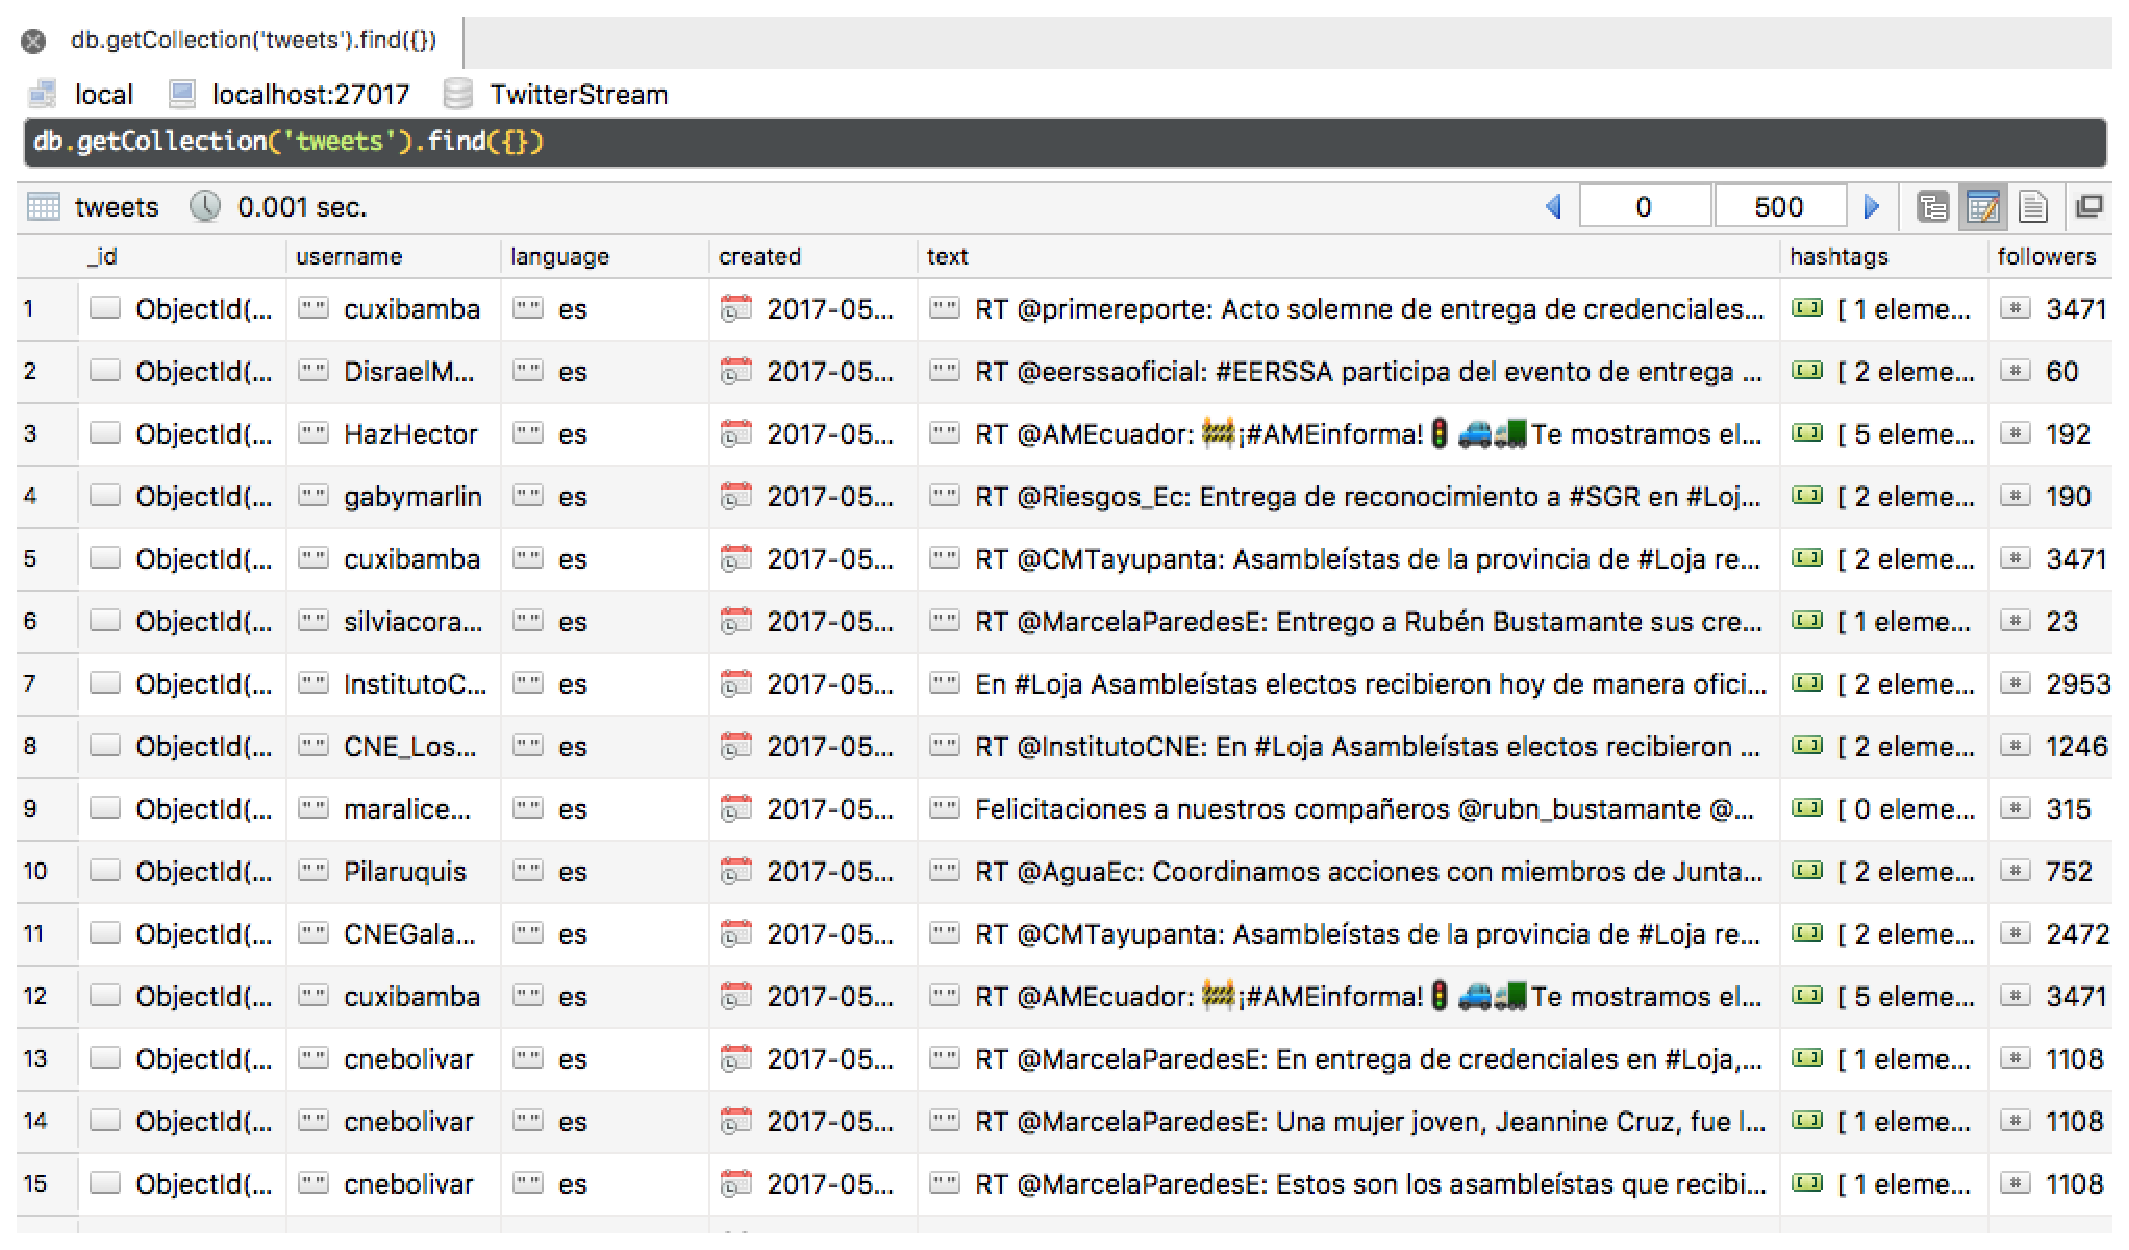
\includegraphics[width=12cm]{tweet_mongo}
\caption{Base MongoDB, tweets extraídos }
\label{fig:dos}
\end{figure}
\begin{itemize}
   \item Para la extracción de datos en Twitter, se utlilizó la librería Tweepy. Esta herramienta mediante un algoritmo escrito en python, permitie la obtención de metadatos de tweets. Los mismos que serán almacenados en una base de datos NoSql " MongoDB", ver Figura \ref{fig:dos}.
    
    
    Los datos que son extraídos corresponden a la ciudad de Loja, para esto el algoritmo fue adaptado para que recolecte los tweets con localización Loja y que además posean la palabra clave Loja, turismoloja, turismo, comida, evento, fiesta,cultura, restaurante, comida, hotel, hostal, alojamiento, fiesta, evento, bar, karaoke, discoteca, parque, iglesia, museo, edificio histórico, gastronomía, festival, sinfónica, viaje, travel,  estadio, partido, carnaval, paisaje, pintura, farra, jipiro, puertadelaciudad, castillo, laguna, lago, montaña, puente, destino, piscina, coliseo, tributo, concierto, arte, artesvivas, artesanía, homenaje, discurso, plaza, cultural, juevescultural, recreación, valle, sagrario, virgen, catedral, libro, feria, invita, teatro, pileta, naturaleza, sendero, reunión, rally, cerro, eólico, excursión, vacaciones, cívico, turista, diacívico, vacación, cueva, biblioteca, cascada, pista, acuario, zoológico, paintball, galería, bosque, jardín, deportes, rifa, bingo, ciclismo, novatada, karting, entre muchos otros. Cabe mencionar que constantemente se estará recolectando tweets con las características antes mencionadas.    
    
\item Por otro lado el catastro turístico de la provincia de Loja,  que tiene registrado el Ministerio de Turismo del Ecuador en formato csv, permitirá encontrar y estructurar de mejor manera la información relacionada a hoteles, restaurantes, recursos turísticos, cada uno con su respectiva ubicación, nombre, teléfono entre otros.


    


\subsection{Tercera Fase}

Se ha modelado la ontología del recomendador turístico en base a la información que se recogerá de las fuentes. En esta se definirán las clases, object properties y data properties, comos se muestra en la Figura \ref{fig:tres}. 

Dentro de las clases identificadas están: 

\begin{multicols}{2} 
\begin{itemize}
    \item Province
        \begin{itemize}
         \item Canton
        \end{itemize}
    \item Person
        \begin{itemize}
         \item Tourist
        \end{itemize}
    \item Organization
        \begin{itemize}
         \item Event
        \end{itemize}
    \item SocialMediaPosting
        \begin{itemize}
         \item UserTweet
    \end{itemize}
    \item Recurso-Turistico
        \begin{itemize}
         \item Museo
         \item Edificio-Histórico
         \item Edificio-Religioso
         \item Entorno-Natural
    \end{itemize}  
    \item Recurso-Hotelero
        \begin{itemize}
         \item Hotel
         \item Hostal
    \end{itemize}
    \item Recurso-Comercial
        \begin{itemize}
         \item Bar
         \item Restaurante
         \item Cafeteria
         \item Discotheque
    \end{itemize}
\end{itemize}
\end{multicols} 

Se han definido las siguientes object properties:
\begin{multicols}{2}
\begin{itemize}
    \item hasCanton
    \item hasHotel
    \item hasHostal
    \item hasBar
    \item hasCafeteria
    \item hasRestaurant
    \item hasDiscotheque
    \item hasMuseum
    \item hasHistoricalBuilding
    \item hasReligiousBuilding
    \item hasNaturalEnviroment
    \item hasEvent
    \item isVisitedBy
    \item subClassOf
    \item about
    \item description
    \item publication
\end{itemize}
\end{multicols}



\begin{figure}
\centering
\includegraphics[width=13cm]{diagrama}
\caption{Diagrama de Clases}
\label{fig:tres}
\end{figure}

Se ha modelado un diseño general de las clases,  object properties y data properties en la herramienta Protégé, como se muestra en la Figura \ref{fig:tres}.

Además se estableció data properties: para recursos turísticos: nombre, latitud y longitud, para recursos comerciales y hoteleros: ubicación y nombre, para eventos: fecha de inicio, descripción y ubicación, para los tweets se usa: fecha de publicación, descripción y palabras claves.

Se detalla características de las propiedades tales como: funcionales, inversas, entre otras, así como restricciones que rigen a las clases como por ejemplo: que en un cantón pueden haber varios recursos de tipo comercial, hotelero o turístico, o que en un evento pueden existir mas de un tweet describiendo el evento.


\end{itemize}
\begin{figure}
\centering
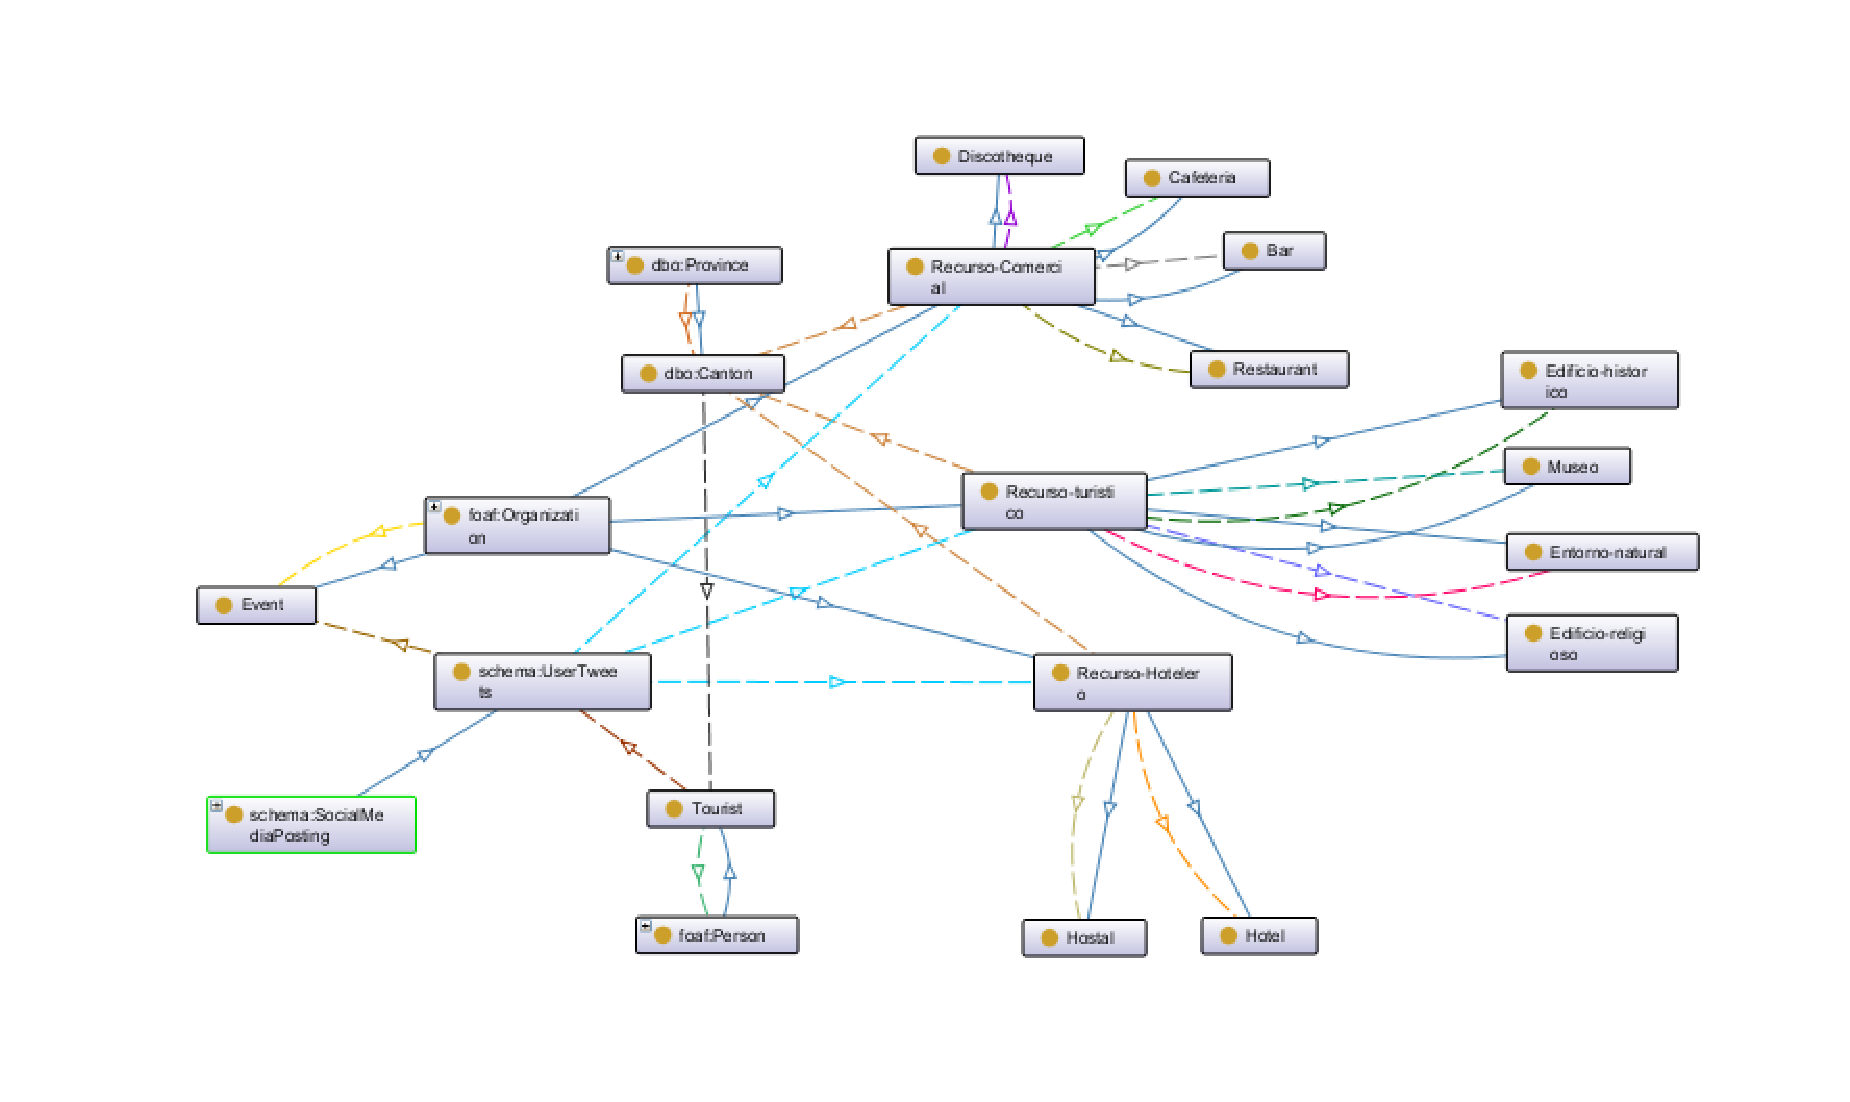
\includegraphics[width=13cm]{protege}
\caption{Ontología para Sistema Recomendador de Turismo en Protégé}
\label{fig:cuatro}
\end{figure}


Para manejar la estructura de la ontología fue necesario utilizar Protégé, ya que permite cargar clases, propiedades, establecer las relaciones necesarias, dominio, rango, etc., generando además un formato de salida como N-triples, turtle, entre otros. Como se observa en la figura \ref{fig:cuatro}.
\section{Resultados}

Se pretende implementar un modelo para la creación de un sistema recomendador de turismo, que se encargue de integrar, vincular la información proporcionada por los usuarios/turistas en Twitter y basado en el catastro  brindado por el Ministerio de Turismo, esta recomendador se orientará a información referente a la provincia de Loja.

La unión de todos estos datos, creará datos enlazados, los cuales darán la opción a los usuarios de obtener información más completa sobre los recursos turísticos de la ciudad de Loja. Se espera usar los datos del catastro como conocimiento base sobre información turística de la ciudad para posteriormente en base  a los tweets recuperados realizar valoraciones de los lugares, hoteles, restaurantes, etc, aportando una mejor experiencia a los turistas

Un sistema recomendador basado en la web semántica, proveerá a las empresas que tengan como fin actividades relacionadas al turismo, poder dar un servicio mucho mejor a todos sus usuarios, y que estos a su vez, logren disfrutar una mejor experiencia durante su estancia en otro lugar.

Esto también beneficiará al país, puesto que aumentará la cantidad de ingresos, además de fomentar el turismo en el mercado nacional e internacional, y servirá de modelo futuro para creación de nuevas aplicaciones, basadas en este modelo.

%
% ---- Bibliography ----
\bibliography{references}{}
\bibliographystyle{acm}
%
\end{document}
